\documentclass[bsc,letterpaper,12pt]{csthesis}
%\documentclass[letter,12pt,twoside]{csthesis}  para imprimir de lado y lado


\paperwidth = 21.6cm		% Tamaño de la hoja
\paperheight = 27.9cm

%Margenes horizontales
\hoffset = -2.54cm		% Se elimna el offset horizontal
\oddsidemargin = 4cm
\evensidemargin = 2cm
\textwidth = 15.6cm

%Margenes verticales
\voffset = 0.46cm
\topmargin = 0cm
\headheight = 0cm
\headsep = 0cm
\textheight = 21.9cm
\footskip = 1.2cm


\usepackage[spanish]{babel}     % Idioma Capitulos y demas
\usepackage[utf8x]{inputenc}
\usepackage[T1]{fontenc}
\usepackage{lmodern}
\usepackage{cc/CreativeCommons}  %Licencia

\usepackage{listings}
\usepackage{verbatim}
\usepackage{moreverb}
\let\verbatiminput=\verbatimtabinput
\def\verbatimtabsize{8}  % Tabulación en verbatim

% Paquete para el manejo de hipervinculos
\usepackage[colorlinks=true,linkcolor=black,urlcolor=black,citecolor=black, urlcolor=black, filecolor=black]{hyperref}

% Paquete para el manejo de tablas
\usepackage{supertabular}
\usepackage{tabularx}

% Paquete para apendices
\usepackage{appendix}

% Paquetes para simbolos
%\usepackage{mathcomp}
%\usepackage{latexsym}
\usepackage{pifont}
\usepackage{amsfonts}
\usepackage{amssymb}
\usepackage{wasysym}
\usepackage{colortbl}
\usepackage{multicol} 
\usepackage{booktabs}

% Manejo de imagenes PDF y EPS
\newif\ifpdf
\ifx\pdfoutput\undefined
\pdffalse % we are not running PDFLaTeX
\else
\pdfoutput=1 % we are running PDFLaTeX
\pdftrue
\fi

\ifpdf
\usepackage[pdftex]{graphicx}
\else
\usepackage{graphicx}
\fi

\ifpdf
\DeclareGraphicsExtensions{.pdf, .jpg, .tif}
\else
\DeclareGraphicsExtensions{.eps, .jpg}
\fi

% Sangria de comienzo de parrafo
\setlength{\parindent}{0cm}
% Espacio vertical entre dos parrfos
\setlength{\parskip}{0.3cm}

% Definir el nombre de listas
\addto\captionsspanish{%
  \def\prefacename{Prefacio}%
  \def\refname{Referencias}%
  \def\abstractname{RESUMEN}%
  \def\bibname{Bibliograf\'ia}%
  \def\chaptername{Cap\'{\i}tulo}%
  \def\listfigurename{LISTA DE FIGURAS}%
  \def\listtablename{LISTA DE CUADROS}%
  \def\indexname{\'Indice alfab\'etico}%
  \def\figurename{Figura}%
  \def\tablename{Tabla}%
  \def\partname{Parte}%
  \def\enclname{Adjunto}%
  \def\ccname{Copia a}%
  \def\headtoname{A}%
  \def\pagename{P\'agina}%
  \def\seename{v\'ease}%
  \def\alsoname{v\'ease tambi\'en}%
  \def\proofname{Demostraci\'on}%
  \def\glossaryname{GLOSARIO}}%
  \def\appendixname{Ap\'endices}%
  \def\appendixtocname{Ap\'endices}%
  \def\appendixpagename{Ap\'endices}%
  \addto\captionsspanish{\def\contentsname{CONTENIDO}}%


% Inico del documento
\begin{document}
\pagestyle{empty}% Sin número de página
%%% PORTADA


\thispagestyle{empty}

\begin{center}{\centering \large BUSCADOR SEMÁNTICO SAWA}
\end{center}

\vspace{4cm}

\begin{center}{\large OMAR ERNESTO CABRERA ROSERO\\ JIMMY MATEO GUERRERO RESTREPO\\ MAURICIO FERNANDO BENAVIDES BENAVIDES \\ SILVIO RICARDO TIMARÁN PEREIRA}
\end{center}

\vspace{1cm}

\begin{figure}[!h]
\begin{center}

\includegraphics[width=4cm]{pictures/udenar.eps}%logo of your university
\end{center}
\end{figure}

\vspace{1cm}

\begin{center}{\large UNIVERSIDAD DE NARIÑO\\
FACULTAD DE INGENIERÍA\\
PROGRAMA DE INGENIERÍA DE SISTEMAS\\
SAN JUAN DE PASTO\\
2014}
\end{center}

\pagebreak


\newpage
\pagestyle{empty}
\section*{Sobre este trabajo}
\CCbyncsaInfo
\tableofcontents

\chapter{Introducción}

La falta de significado que se maneja en la Web actual, dificulta la 
búsqueda eficiente de información. La web semántica ha comenzado a adquirir una
gran importancia debido a que se quiere encontrar información de manera precisa  y 
poder convertirla en información del conocimiento y representarla en recursos web que
puedan estar disponibles en otras aplicaciones. Para lograr encontrar un significado
claro en la búsqueda,  la Web semántica hace uso de ontologías, que organizan la 
información de manera que se podrá interpretar lo que se quiere buscar y, por tanto, 
permitirá buscar e integrar datos mucho mejor que ahora.

Esta aplicación web soporta la búsqueda
inteligente de los trabajos de grado de la Universidad de Nariño mediante una ontología
de aplicación.
\chapter{Contrucción de la aplicación}

El buscador semántico SAWA fue desarrollado en JavaEE\footnote{Java Platform, Enterprise Edition o Java EE
(anteriormente conocido como Java 2 Platform, Enterprise Edition o J2EE hasta la versión 1.4}
y liberado bajo licencia libre GPL3\footnote{\url{http://www.gnu.org/licenses/gpl.html}} el cual puede 
ser descargado del repositorio del portal github\footnote{\url{https://github.com/poldrosky/Sawa}} y
se puede mirar el funcionamiento en la página\footnote{\url{http://ingenieria.udenar.edu.co:8080/Sawa/}}. 

En la aplicación se usaron algoritmos  como lematizadores y similitud de palabras 
para hacer corrección ortográfica, en caso de que el usuario tenga error de digitación,
además de la construcción de un tesauro para que pueda hacer la búsqueda por sinónimos
de palabras.

Las siguientes son las características específicas del software construido:

\begin{itemize}
 \item Búsqueda General.
 \item Búsqueda por título.
 \item Búsqueda por autor.
 \item Auto completar palabras.
 \item Corrección de digitación.
 \item Búsqueda por sinónimos.
 \item Ordenamiento de resultados por mayor coincidencia.
\end{itemize}

En el diagrama de actividades de la Figura~\ref{figura:prueba1}  
se muestra como se realiza una búsqueda.

\begin{figure}[!ht]
\begin{center}
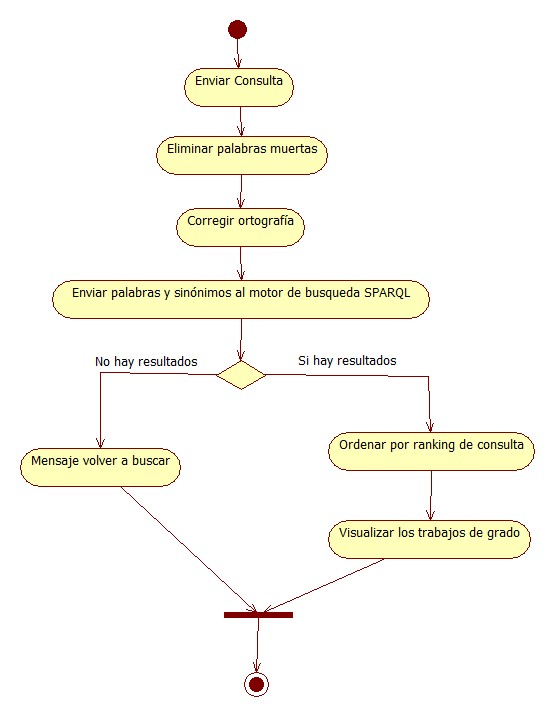
\includegraphics[width=10cm]{pictures/prueba1.jpg}
\end{center}
\caption{Diagrama de actividades de la búsqueda} \label{figura:prueba1}
\end{figure}


Para la construcción del software se tubo en cuenta la manera de 
realizar las consultas usando el lenguaje SPARQL y la extensión de 
postgresql pg\_similarity\footnote{\url{http://pgsimilarity.projects.pgfoundry.org}}.
\chapter{Funcionamiento de la Aplicación}

Para la aplicación de las pruebas se realizaron siete casos de prueba con diez iteraciones
cada una, para ver la eficiencia del buscador desarrollado y el actual
buscador de la biblioteca de la Universidad de Nariño\footnote{\url{http://biblioteca.udenar.edu.co:8085/bibliotecavirtual/}}.

Las pruebas se hicieron llevando los siguientes casos de prueba y se calificó
como éxito (E) o fracaso (F), teniendo en cuenta que el éxito se lo califica si
la búsqueda a realizar está en los quince primeros resultados.

\subsection{Casos de prueba}

\begin{description}
 \item [Búsqueda por título completo:] esta búsqueda se la realizó enviando la consulta con 
 el título exacto que aparece en la base de datos(tildes, signos de puntuación y comillas), dando como
 resultado que los dos sistemas se comportan de la misma manera como lo muestra la Tabla~\ref{tabla:p1} y Figura~\ref{figura:p1}.
 
 \begin{center}
\begin{table}[!ht]
\caption{Búsqueda por título completo} \label{tabla:p1}
\scalebox{0.7}{
\begin{tabular}{|p{1cm} | p{14cm} | p{1.5cm} | p{2cm} |}
\toprule
\textbf{No} & \textbf{Consulta} & \textbf{SAWA} & \textbf{Biblioteca} \\
\hline
 1 & MATE-KDD: UNA HERRAMIENTA GENERICA PARA EL DESCUBRIMIENTO DE REGLAS DE CLASIFICACION MEDIANAMENTE ACOPLADA AL SGBD POSTGRESQL & E & E \\
 \hline
 2 & TARIYKDD : UNA HERRAMIENTA GENERICA DE DESCUBRIMIENTO DE CONOCIMIENTO EN BASES DE DATOS DEBILMENTE ACOPLADA CON EL SGBD POSTGRESQL & E & E \\
 \hline
 3 & IMPLANTACION DE PRIMITIVAS SQL PARA EL DESCUBRIMIENTO DE REGLAS DE ASOCIACION Y CLASIFICACION & E & E \\
 \hline
 4 & ATLAS HERRAMIENTA DE CARTOGRAFIA WEB Y GEOCODIFICACION PARA EL DESARROLLO DE SISTEMAS HIBRIDOS EN AREAS URBANAS SOBRE J2EE Y POSTGRESQL & E & E\\
 \hline
 5 & GEOPASTO UN SISTEMA DE INFORMACION GEOGRAFICA WEB ORIENTADO AL APOYO PARA LA TOMA DE DECISIONES BASADOS EN EL PLAN DE ORDENAMIENTO TERRITORIAL & E & E \\
 \hline
 6 & SISTEMA DE INFORMACION PARA EL REGISTRO Y CONSULTA DEL MATERIAL DE BIBLIOTECA EN EL ENTORNO INTRANET DEL CENTRO SUR COLOMBIANO DE LOGISTICA INTERNACIONAL & E & E\\
 \hline
 7 & SISTEMA DE INFORMACION PARA LA BIBLIOTECA Y DESARROLLO DE LA PAGINA WEB DE LA UNIVERSIDAD DE NARIÑO -SEDE IPIALES & E & E\\
 \hline
 8 & ANALISIS, DISEÑO Y DESARROLLO DE UN SISTEMA DE INFORMACION MEDIANTE UNA RED DE COMUNICACIONES E INTERNET PARA LA ALCALDIA DE LINARES. & E & E\\
 \hline
 9 & SISTEMA DE INFORMACION PARA EL MANEJO CONTABLE DE LOS ALMACENES DEL GRUPO CABAL IPIALES & E& E\\
 \hline
 10 & DESARROLLO DE UN SISTEMA DE INFORMACION COMPUTARIZADO DE REGISTRO Y CONTROL ACADEMICO PARA EL POLITECNICO SAN JUAN DE PASTO & E& E\\
 \hline
\midrule
\bottomrule
\end{tabular}
}
\end{table}
\end{center}
 
 \begin{figure}[!ht]
\begin{center}
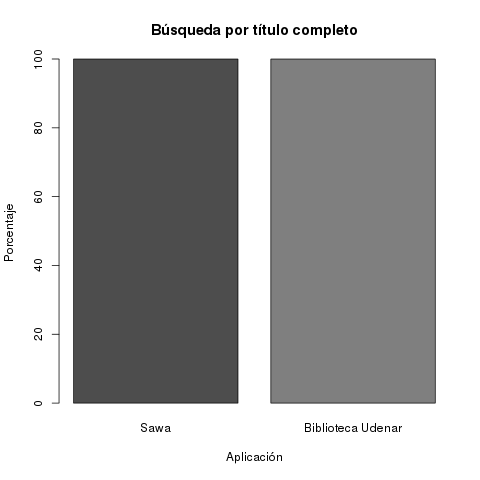
\includegraphics[width=8cm]{pictures/p1.png}
\end{center}
\caption{Búsqueda por título completo} \label{figura:p1}
\end{figure}

\newpage
  
 \item [Búsqueda por autor completo:] esta búsqueda se la realizó enviando la consulta con
 el autor exacto que aparece en la base de datos, dando como resultado que el sistema realizado
 en esta investigación de un resultado del 100\% y el sistema de biblioteca 40\% como lo muestra la Tabla~\ref{tabla:p2} y Figura~\ref{figura:p2}.
 
  \begin{center}
\begin{table}[!ht]
\caption{Búsqueda por autor completo} \label{tabla:p2}
\scalebox{0.7}{
\begin{tabular}{|c|l |c| c|}
\toprule
\textbf{No} & \textbf{Consulta} & \textbf{SAWA} & \textbf{Biblioteca} \\
\hline
 1 & CLAUDIA MILENA CASTRO RODRIGUEZ & E & F \\
 \hline
 2 & ANDRES OSWALDO CALDERON ROMERO & E & E \\
 \hline
 3 & STIVENSON ARMERO KREISBERGER & E & E \\
 \hline
 4 & CARLOS ERNESTO ARTEAGA NOGUERA & E & F \\
 \hline
 5 & JUAN CARLOS ROMAN FIGUEROA & E & E\\
 \hline
 6 & HECTOR EDMUNDO ROSERO CASTRO & E & F \\
 \hline
 7 & PAOLA MARY CORAL BASTIDAS & E & F\\
 \hline
 8 & OCTAVIO DELGADO ORDOÑEZ & E & E\\
 \hline
 9 & MARIA ELENA ESTRADA ESPAÑA & E & F\\
 \hline
 10 & YEIMY ANDRES ARTEAGA GUERRON& E& F\\
 \hline
\midrule
\bottomrule
\end{tabular}
}
\end{table}
\end{center}
 
 \begin{figure}[!ht]
\begin{center}
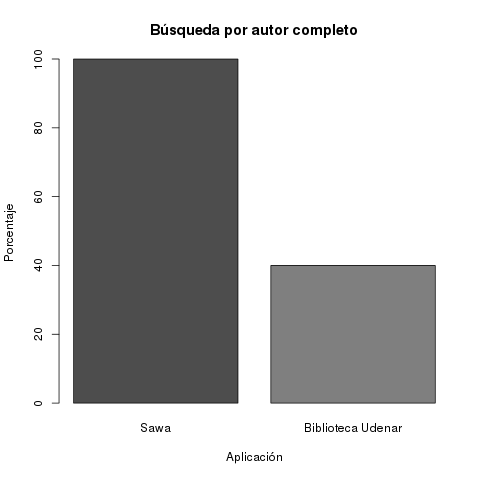
\includegraphics[width=8cm]{pictures/p2.png}
\end{center}
\caption{Búsqueda por autor completo} \label{figura:p2}
\end{figure}
 
 \newpage
 \item [Búsqueda por un nombre y un apellido:] esta búsqueda se la realizó enviando la consulta
 con un nombre y un autor unicamente, dando como resultado que el sitema realizado
 en esta investigación de un resultado del 90\% y el sistema de biblioteca 40\% como lo muestra la Tabla~\ref{tabla:p3} y Figura~\ref{figura:p3}.
 
  \begin{center}
\begin{table}[!ht]
\caption{Búsqueda por un nombre y un apellido} \label{tabla:p3}
\scalebox{0.7}{
\begin{tabular}{|c|l |c| c|}
\toprule
\textbf{No} & \textbf{Consulta} & \textbf{SAWA} & \textbf{Biblioteca} \\
\hline
 1 & CLAUDIA  RODRIGUEZ & E & F \\
 \hline
 2 & ANDRES CALDERON & E & E \\
 \hline
 3 & STIVENSON KREISBERGER & E & E \\
 \hline
 4 & CARLOS   NOGUERA & E & F \\
 \hline
 5 & JUAN FIGUEROA & E & E\\
 \hline
 6 & HECTOR  ROSERO & E & F \\
 \hline
 7 & MARY CORAL & E & F\\
 \hline
 8 & OCTAVIO DELGADO & E & E\\
 \hline
 9 & ELENA  ESPAÑA & F & F\\
 \hline
 10 & YEIMY  ARTEAGA & E& F\\
 \hline
\midrule
\bottomrule
\end{tabular}
}
\end{table}
\end{center}
 
 \begin{figure}[!ht]
\begin{center}
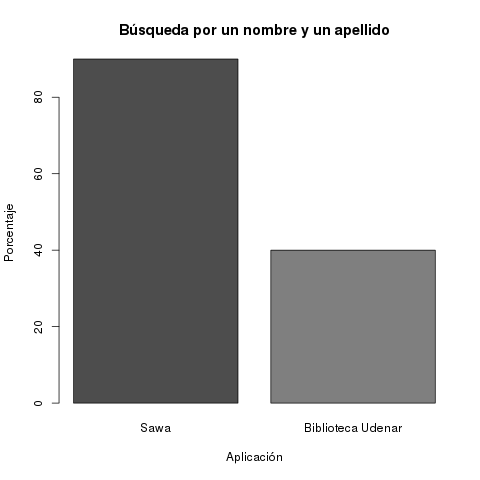
\includegraphics[width=8cm]{pictures/p3.png}
\end{center}
\caption{Búsqueda por un nombre y un apellido} \label{figura:p3}
\end{figure}
 
 \newpage
 \item [Búsqueda por palabras contenidas en el título:] esta búsqueda se la realizó enviando la consulta
 con palabras que estén contenidas en el título, las palabras podían haberse enviado en el ordén del
 título como en desorden, dando como resultado que el sitema realizado
 en esta investigación de un resultado del 100\% y el sistema de biblioteca 0\% como lo muestra la Tabla~\ref{tabla:p4} y Figura~\ref{figura:p4}.
 
    \begin{center}
\begin{table}[!ht]
\caption{Búsqueda por palabras contenidas en el título}  \label{tabla:p4}
\scalebox{0.7}{
\begin{tabular}{|c|l |c| c|}
\toprule
\textbf{No} & \textbf{Consulta} & \textbf{SAWA} & \textbf{Biblioteca} \\
\hline
 1 & REGLAS GENERICAS DE CLASIFICACION & E & F \\
 \hline
 2 & CONOCIMIENTO ACOPLADO A UNA BASE DE DATOS & E & F \\
 \hline
 3 & PRIMITIVAS PARA EL DESCUBRIMIENTO DE REGLAS & E & F \\
 \hline
 4 & CARTOGRAFIA Y GEOCODIFICACION WEB & E & F\\
 \hline
 5 & GEOPASTO ORIENTADO ALA TOMA DE DECISIONES & E & F \\
 \hline
 6 & REGISTRO  DEL MATERIAL DE BIBLIOTECA & E & F\\
 \hline
 7 & DESARROLLO DEL SISTEMA  PARA LA BIBLIOTECA & E & F\\
 \hline
 8 & ANALISIS Y DESARROLLO DE UNA UNA RED DE COMUNICACIONES & E & F\\
 \hline
 9 & SISTEMA PARA EL MANEJO CONTABLE DEL GRUPO CABAL & E& F\\
 \hline
 10 & SISTEMA DE INFORMACION DE REGISTRO Y CONTROL ACADEMICO & E& F\\
 \hline
\midrule
\bottomrule
\end{tabular}
}
\end{table}
\end{center}
 
  \begin{figure}[!ht]
\begin{center}
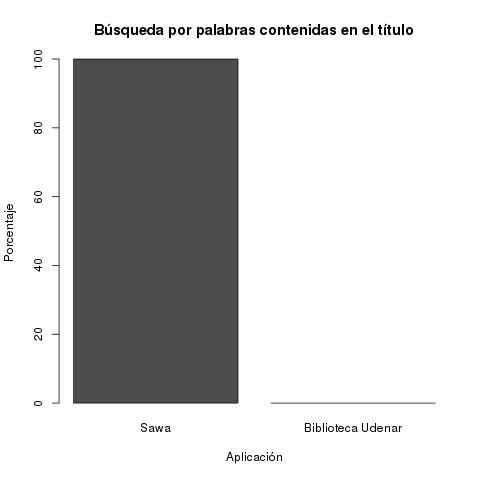
\includegraphics[width=8cm]{pictures/p4.png}
\end{center}
\caption{Búsqueda por palabras contenidas en el título} \label{figura:p4}
\end{figure}
 
 \newpage
 \item [Búsqueda por error ortográfico en el título:] esta búsqueda se la realizó enviando la consulta
 con uno o dos errores de digitación en el título, dando como resultado que el sitema realizado
 en esta investigación de un resultado del 100\% y el sistema de biblioteca 0\% como lo muestra la Tabla~\ref{tabla:p5} y Figura~\ref{figura:p5}.
 
 \begin{center}
\begin{table}[!ht]
\caption{Búsqueda por error ortográfico en el título} \label{tabla:p5}
\scalebox{0.7}{
\begin{tabular}{|p{1cm} | p{14cm} | p{1.5cm} | p{2cm} |}
\toprule
\textbf{No} & \textbf{Consulta} & \textbf{SAWA} & \textbf{Biblioteca} \\
\hline
 1 & MATE-KDD UNA HERRAMIENTA GENERICA PARA EL DESCUBRIMIENTO DE REGLOS DE CLASIFICACION MEDIANAMENTE ACOPLADA AL SGBD POSTGRESQL & E & F \\
 \hline
 2 & TARIYKDD UNA HERRAMIENTA GENERICA DE DESCUBRIMIENTO DE CONOCIMENTO EN BASES DE DATOS DEBILMENTE ACOPLADA CON EL SGBD POSTGRESQL & E & F\\
 \hline
 3 & IMPLANTACION DE PRIMITIVAS SQL PARA EL DESCUBRIMINTO DE REGLAS DE ASOSIASION Y CLASIFICACION & E & F \\
 \hline
 4 & ATLAS HERRAMIENTA DE CARTOGAFIA WEB Y GEOCODIFICACION PARA EL DESARROLLO DE SISTEMAS HIBRIDOS EN AREAS URBANAS SOBRE JEE Y POSTGRES & E & F\\
 \hline
 5 & GEOPATO UN SISTEMA DE INFORMACION GEOGAFICA WEB ORIENTADO AL APOYO PARA LA TOMA DE DECISIONES BASADOS EN EL PLAN DE ORDENAMIENTO TERRITORIAL & E & F \\
 \hline
 6 & SISTEMA DE INFORMACIOM PARA EL REGISTRO Y CONSULT DEL MATERIAL DE BIBLIOTECA EN EL ENTORNO INTRANET DEL CENTRO SUR COLOMBIANO DE LOGISTICA INTERNACIONAL & E & F\\
 \hline
 7 & SISTEMA DE INFORMACION PARA LA BIBLIOTECA Y DESARROLLO DE LA PAGINA WEB DE LA UNIVERSIDAD DE NARINO IPIALES & E & F\\
 \hline
 8 & ANALISIS DISENO Y DESARROLLO DE UN SISTEMA DE INFORMACION MEDIANTE UNA RED DE COMUNICASIONES E INTERNET PARA LA ALCALDIA DE LINARES. & E & F\\
 \hline
 9 & SISTEMA DE INFORMACION PARA EL MANEJO CONTABE DE LOS ALMASENES DEL GRUPO CABAL IPIALES & E& F\\
 \hline
 10 & DESARROLLO DE UN SISTEMA DE INFORMACION COMPUTALIZADO DE REGISTRO Y CONTROL ACADEMIC PARA EL POLITENICO SAN JUAN DE PASTO & E& F\\
 \hline
\midrule
\bottomrule
\end{tabular}
}
\end{table}
\end{center}
 
  
  \begin{figure}[!ht]
\begin{center}
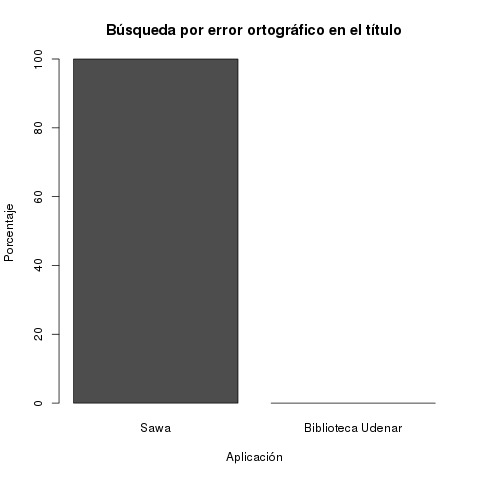
\includegraphics[width=8cm]{pictures/p5.png}
\end{center}
\caption{Búsqueda por error ortográfico en el título} \label{figura:p5}
\end{figure}

 \newpage
 \item [Búsqueda por error ortográfico en el autor:] esta búsqueda se la realizó enviando la consulta
 con uno o dos errores de digitación en el auto, dando como resultado que el sitema realizado
 en esta investigación de un resultado del 100\% y el sistema de biblioteca 0\% como lo muestra la Tabla~\ref{tabla:p6} y Figura~\ref{figura:p6}.
 
  \begin{center}
\begin{table}[!ht]
\caption{Búsqueda por error ortográfico en el autor} \label{tabla:p6}
\scalebox{0.7}{
\begin{tabular}{|c|l |c| c|}
\toprule
\textbf{No} & \textbf{Consulta} & \textbf{SAWA} & \textbf{Biblioteca} \\
\hline
 1 & CLAUDA MILENA CASTRO RODRIGUEZ & E & F \\
 \hline
 2 & ANDES OSWALDO CALDEROM ROMERO & E & F \\
 \hline
 3 & STIVENSOM ARMERA KREISBERGER & E & F\\
 \hline
 4 & CARLOS ERNESSTO ATEAGA NOGUERA & E & F \\
 \hline
 5 & JUAN CARLS ROMAM FIGUEROA & E & F\\
 \hline
 6 & ECTOR EDMUDO ROSERO CASTRO & E & F \\
 \hline
 7 & PAOA MARYS CORAL BASTIDAS & E & F\\
 \hline
 8 & OCTAIO DELGADO ORDOÑEZ & E & F\\
 \hline
 9 & MARA ELENA ESTADA ESPAÑA & E & F\\
 \hline
 10 & YEIMMY ANDRESS ARTEAGA GUERRON& E& F\\
 \hline
\midrule
\bottomrule
\end{tabular}
}
\end{table}
\end{center}
 
   \begin{figure}[!ht]
\begin{center}
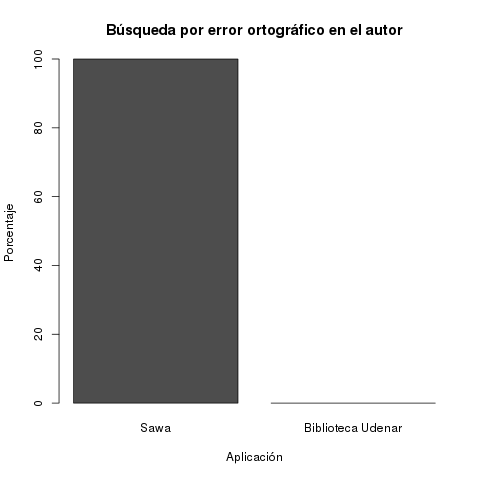
\includegraphics[width=8cm]{pictures/p6.png}
\end{center}
\caption{Búsqueda por error ortográfico en el autor} \label{figura:p6}
\end{figure}

\newpage
 \item [Búsqueda por sinónimos de palabras:] esta búsqueda se la realizó enviando la consulta con algunos de los
 sinónimos de palabras contenidas en el título,  dando como resultado que el sitema realizado
 en esta investigación de un resultado del 80\% y el sistema de biblioteca 0\% como lo muestra la Tabla~\ref{tabla:p7} y Figura~\ref{figura:p7}.
 
 \begin{center}
\begin{table}[!ht]
\caption{Búsqueda por sinónimos de palabras}  \label{tabla:p7}
\scalebox{0.7}{
\begin{tabular}{|c|l |c| c|}
\toprule
\textbf{No} & \textbf{Consulta} & \textbf{SAWA} & \textbf{Biblioteca} \\
\hline
 1 & entendimiento adaptado a una  base bases datos& E & F \\
 \hline
 2 &  intrumento de hallazgo para conocer & E & F \\
 \hline
 3 & elemental hallazgo DE REGLAS & E & F \\
 \hline
 4 & georreferenciación y localización web & E & F\\
 \hline
 5 & geopasto poner tomas de determinación & E & F \\
 \hline
 6 & inspección e informe de archivo o biblioteca & E & F\\
 \hline
 7 & creacion del sistema  para archivo & E & F\\
 \hline
 8 & estudio y creacion de un a red de comunicado & F & F\\
 \hline
 9 & empleo de la asociación cabal& F& F\\
 \hline
 10 & desarrollo de un sistema de inspección para el control escolar & E& F\\
 \hline
\midrule
\bottomrule
\end{tabular}
}
\end{table}
\end{center}
 
   \begin{figure}[!ht]
\begin{center}
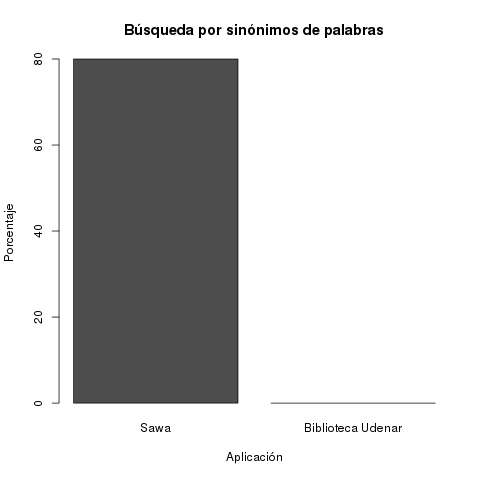
\includegraphics[width=8cm]{pictures/p7.png}
\end{center}
\caption{Búsqueda por sinónimos de palabras} \label{figura:p7}
\end{figure}
 
\end{description}


Se puede mirar el funcionamiento del software y como fueron ejecutadas las pruebas
en el video adjunto  (``Documentacion/Pruebas.mp4'') o en línea\footnote{\url{http://www.youtube.com/watch?v=niE-FcWzp6Q}}.




 
\chapter{Instalación de la aplicación}

Para poder instalar la aplicación debemos instalar PostgreSQL 9.1, Glassfish 3.1.2.2 y la extensión
para postgresql llamada pg\_similarity, la aplicación solo puede ser instalada bajo sistemas
operativos GNU/Linux


Para la instalación de PostgreSQL 9.1 (Para Debian/Linux), en una terminal se ejecuta los siguiente:\\

\lstset{backgroundcolor=\color{white},frame=shadowbox, basicstyle=\small,  breaklines=true, breaklines=true,language=bash}
\begin{lstlisting}
$ su
# apt-get install postgresql postgresql-client pgadmin3
postgresql-server-dev-all postgresql-contrib
\end{lstlisting}

Ahora se borra la contraseña para la cuenta de  administrador de ``postgres'' para ello se ejecuta lo
siguiente en la linea de comandos. \\

\lstset{backgroundcolor=\color{white},frame=shadowbox, basicstyle=\small,  breaklines=true, breaklines=true,language=bash}
\begin{lstlisting}
# su postgres -c psql template1
\end{lstlisting}

\lstset{backgroundcolor=\color{white},frame=shadowbox, basicstyle=\small,  breaklines=true, breaklines=true,language=sql}
\begin{lstlisting}
template1=# ALTER USER postgres WITH PASSWORD `postgres1';
template1=#\q
\end{lstlisting}

Eso altera la contraseña dentro de la base de datos, ahora se tiene que hacer lo mismo para el  
usuario 'postgres' y colocar la misma contraseña que utilizó anteriormente. \\

\lstset{backgroundcolor=\color{white},frame=shadowbox, basicstyle=\small,  breaklines=true, breaklines=true,language=bash}
\begin{lstlisting}
# passwd -d postgres
 #su postgres -c passwd
\end{lstlisting}

Ahora para instalar pg\_similarity primero se descarga desde github de la siguiente manera

\lstset{backgroundcolor=\color{white},frame=shadowbox, basicstyle=\small,  breaklines=true, breaklines=true,language=bash}
\begin{lstlisting}
$ git clone https://github.com/eulerto/pg_similarity.git 
\end{lstlisting}

Luego para que pueda ser usada la extensión se la compila como superusuario de la siguiente manera.

\lstset{backgroundcolor=\color{white},frame=shadowbox, basicstyle=\small,  breaklines=true, breaklines=true,language=bash}
\begin{lstlisting}
# su
# cd pg_similarity
# USE_PGXS=1 make
# USE_PGXS=1 make install
# su postgres
$ createdb sawa
\end{lstlisting}

Luego se crea las funciones y se restaura la copia de la base de datos sawa.sql

\lstset{backgroundcolor=\color{white},frame=shadowbox, basicstyle=\small,  breaklines=true, breaklines=true,language=bash}
\begin{lstlisting}
$ psql sawa
sawa=# create extension pg_similarity;
sawa=# \i sawa.sql
\end{lstlisting}

\textbf{Instalación de Glassfish}

Primero se descarga la versión 3.1.2.2 para GNU/linux desde la página de Oracle\footnote{http://www.oracle.com/technetwork/middleware/glassfish/downloads/ogs-3-1-1-downloads-439803.html}
y se la ejecuta.

\lstset{backgroundcolor=\color{white},frame=shadowbox, basicstyle=\small,  breaklines=true, breaklines=true,language=bash}
\begin{lstlisting}
$ sh ogs-3.1.2.2-unix-ml.sh
\end{lstlisting}

Hay que descargar el driver JDBC de postgresql desde la 
página de PostgreSQL\footnote{http://jdbc.postgresql.org} y copiarlo en 
el directorio glassfish3/glassfish/domains/domain1/lib. Para iniciar el servidor 
se ejecuta lo siguiente


\lstset{backgroundcolor=\color{white},frame=shadowbox, basicstyle=\small,  breaklines=true, breaklines=true,language=bash}
\begin{lstlisting}
$ ./glassfish3/glassfish/bin/startserv
\end{lstlisting}

Con esto ya en en el navegador se inglesa con la dirección http://localhost:8080, y
entramos a la consola de administración, ingresamos usuario y contraseña de haber escrito una
en la instalación de glassfish.

Ir  a ``Resources/JDBC/Connection Pools'' y crear una nueva conexión con los datos que muestra la
Figura~\ref{figura:m1} y luego clic en siguiente.

\begin{figure}[!ht]
\begin{center}
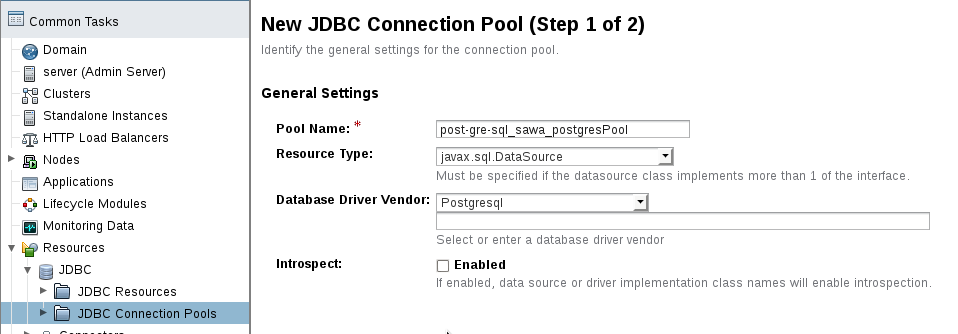
\includegraphics[width=13cm]{pictures/m1.png}
\end{center}
\caption{Crear Nueva conexión} \label{figura:m1}
\end{figure}

Seleccione el origen de datos de nombre de clase org.postgresql.ds.PGConnectionPoolDataSource 
y escribir a las siguientes propiedades adicionales como muestra la Figura~\ref{figura:m2}.

\begin{figure}[!ht]
\begin{center}
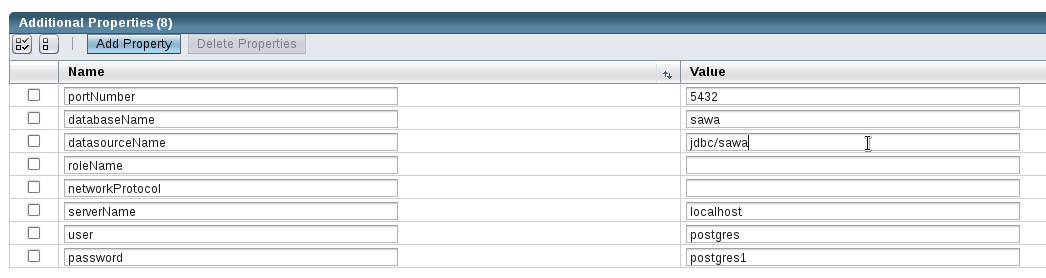
\includegraphics[width=13cm]{pictures/m2.png}
\end{center}
\caption{Propiedades adicionales de conexión} \label{figura:m2}
\end{figure}

Ya con esto guardamos las conexiones y damos clic en finalizar para guardar la conexión.

Luego en ``Resources/JDBC/JDBC Resources'' escribimos en nombre JNDI y escogemos el Pool Name creado 
anteriormente como lo muestra la  Figura~\ref{figura:m3}.

\begin{figure}[!ht]
\begin{center}
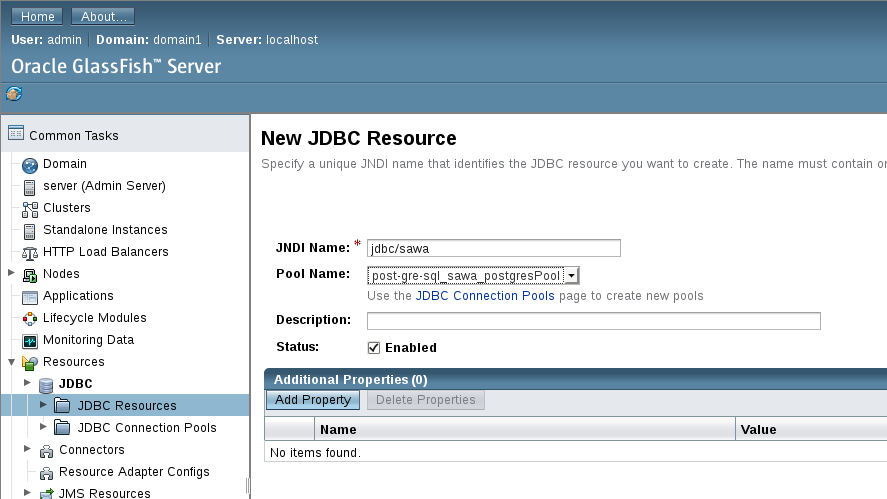
\includegraphics[width=13cm]{pictures/m3.png}
\end{center}
\caption{Recursos JDBC} \label{figura:m3}
\end{figure}

Ya por último en ``Applications'' escogemos en donde tenemos almacenada la aplicación web 
que tiene extensión ``.war'' como muestra la  Figura~\ref{figura:m4}.

\begin{figure}[!ht]
\begin{center}
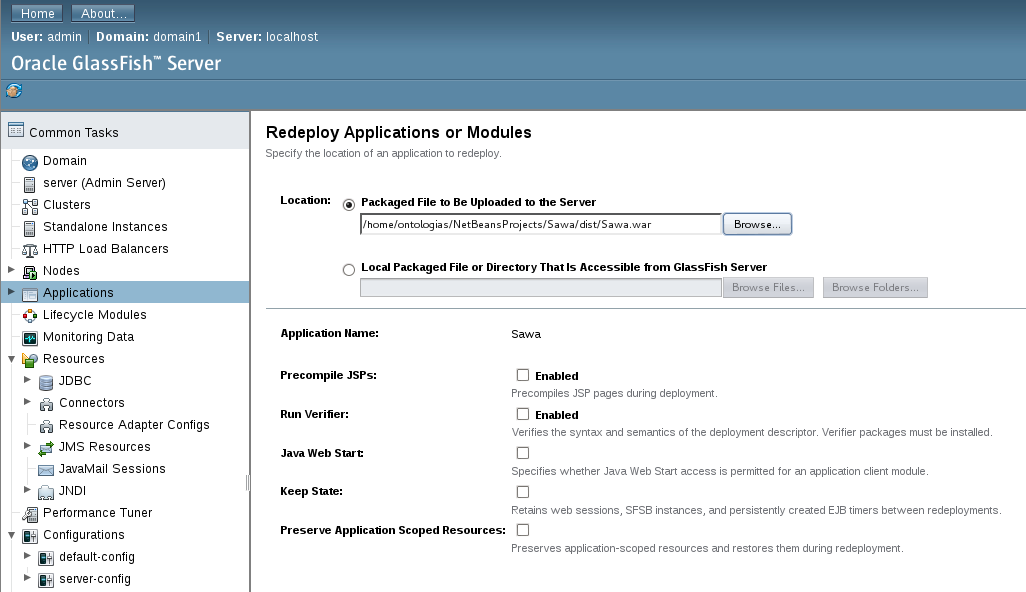
\includegraphics[width=13cm]{pictures/m4.png}
\end{center}
\caption{Subir Aplicación} \label{figura:m4}
\end{figure}

Si todo sale bien nos aparecerá una ventana con la url de la aplicación 
como muestra la Figura~\ref{figura:m5}. y al 
ingresar a la aplicación nos desplegara la ventana de inicio de la aplicación como lo muestra la
Figura~\ref{figura:m6}.

\begin{figure}[!ht]
\begin{center}
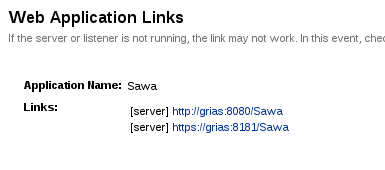
\includegraphics[width=10cm]{pictures/m5.png}
\end{center}
\caption{Url de la Aplicación} \label{figura:m5}
\end{figure}

\begin{figure}[!ht]
\begin{center}
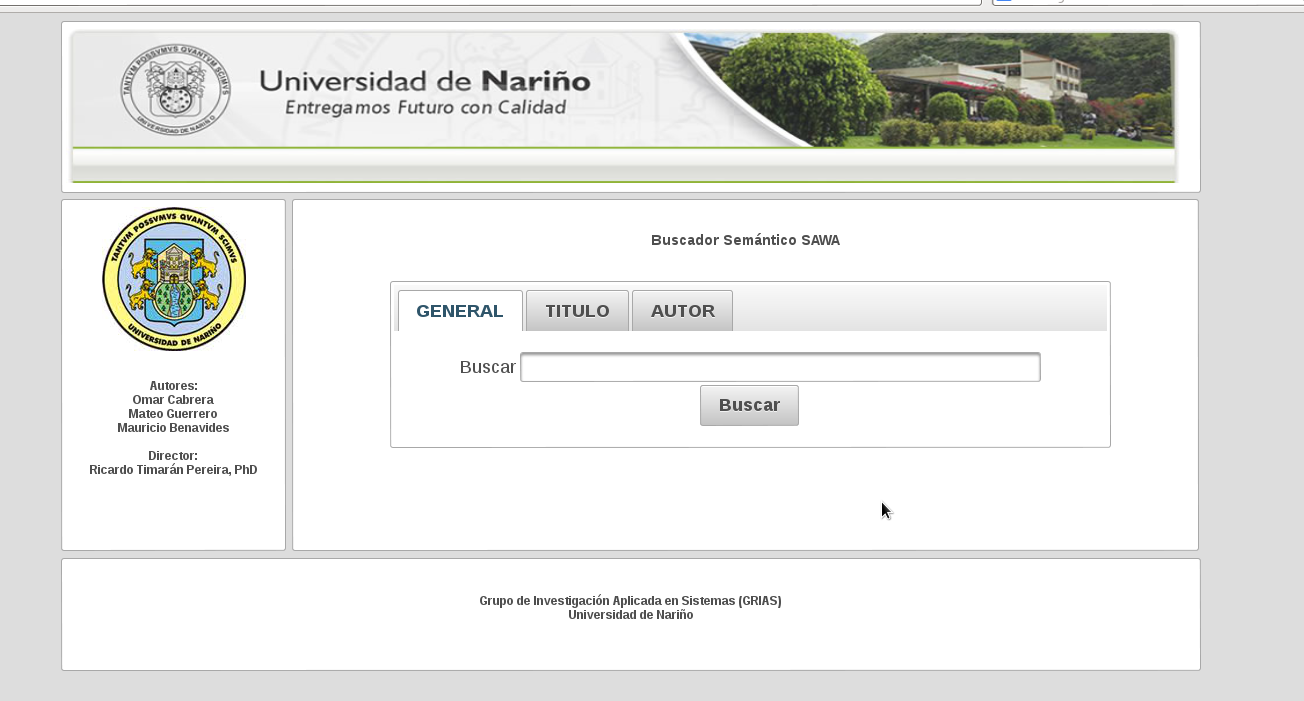
\includegraphics[width=13cm]{pictures/m6.png}
\end{center}
\caption{Aplicación} \label{figura:m6}
\end{figure}

La aplicación esta alojada en \url{http://ingenieria.udenar.edu.co:8080/Sawa/}


 

\end{document}

